\documentclass[twoside]{book}

% Packages required by doxygen
\usepackage{fixltx2e}
\usepackage{calc}
\usepackage{doxygen}
\usepackage[export]{adjustbox} % also loads graphicx
\usepackage{graphicx}
\usepackage[utf8]{inputenc}
\usepackage{makeidx}
\usepackage{multicol}
\usepackage{multirow}
\PassOptionsToPackage{warn}{textcomp}
\usepackage{textcomp}
\usepackage[nointegrals]{wasysym}
\usepackage[table]{xcolor}

% Font selection
\usepackage[T1]{fontenc}
\usepackage[scaled=.90]{helvet}
\usepackage{courier}
\usepackage{amssymb}
\usepackage{sectsty}
\renewcommand{\familydefault}{\sfdefault}
\allsectionsfont{%
  \fontseries{bc}\selectfont%
  \color{darkgray}%
}
\renewcommand{\DoxyLabelFont}{%
  \fontseries{bc}\selectfont%
  \color{darkgray}%
}
\newcommand{\+}{\discretionary{\mbox{\scriptsize$\hookleftarrow$}}{}{}}

% Page & text layout
\usepackage{geometry}
\geometry{%
  a4paper,%
  top=2.5cm,%
  bottom=2.5cm,%
  left=2.5cm,%
  right=2.5cm%
}
\tolerance=750
\hfuzz=15pt
\hbadness=750
\setlength{\emergencystretch}{15pt}
\setlength{\parindent}{0cm}
\setlength{\parskip}{0.2cm}
\makeatletter
\renewcommand{\paragraph}{%
  \@startsection{paragraph}{4}{0ex}{-1.0ex}{1.0ex}{%
    \normalfont\normalsize\bfseries\SS@parafont%
  }%
}
\renewcommand{\subparagraph}{%
  \@startsection{subparagraph}{5}{0ex}{-1.0ex}{1.0ex}{%
    \normalfont\normalsize\bfseries\SS@subparafont%
  }%
}
\makeatother

% Headers & footers
\usepackage{fancyhdr}
\pagestyle{fancyplain}
\fancyhead[LE]{\fancyplain{}{\bfseries\thepage}}
\fancyhead[CE]{\fancyplain{}{}}
\fancyhead[RE]{\fancyplain{}{\bfseries\leftmark}}
\fancyhead[LO]{\fancyplain{}{\bfseries\rightmark}}
\fancyhead[CO]{\fancyplain{}{}}
\fancyhead[RO]{\fancyplain{}{\bfseries\thepage}}
\fancyfoot[LE]{\fancyplain{}{}}
\fancyfoot[CE]{\fancyplain{}{}}
\fancyfoot[RE]{\fancyplain{}{\bfseries\scriptsize Generated on Wed Mar 23 2016 13\+:14\+:22 for Robot by Doxygen }}
\fancyfoot[LO]{\fancyplain{}{\bfseries\scriptsize Generated on Wed Mar 23 2016 13\+:14\+:22 for Robot by Doxygen }}
\fancyfoot[CO]{\fancyplain{}{}}
\fancyfoot[RO]{\fancyplain{}{}}
\renewcommand{\footrulewidth}{0.4pt}
\renewcommand{\chaptermark}[1]{%
  \markboth{#1}{}%
}
\renewcommand{\sectionmark}[1]{%
  \markright{\thesection\ #1}%
}

% Indices & bibliography
\usepackage{natbib}
\usepackage[titles]{tocloft}
\setcounter{tocdepth}{3}
\setcounter{secnumdepth}{5}
\makeindex

% Hyperlinks (required, but should be loaded last)
\usepackage{ifpdf}
\ifpdf
  \usepackage[pdftex,pagebackref=true]{hyperref}
\else
  \usepackage[ps2pdf,pagebackref=true]{hyperref}
\fi
\hypersetup{%
  colorlinks=true,%
  linkcolor=blue,%
  citecolor=blue,%
  unicode%
}

% Custom commands
\newcommand{\clearemptydoublepage}{%
  \newpage{\pagestyle{empty}\cleardoublepage}%
}


%===== C O N T E N T S =====

\begin{document}

% Titlepage & ToC
\hypersetup{pageanchor=false,
             bookmarks=true,
             bookmarksnumbered=true,
             pdfencoding=unicode
            }
\pagenumbering{roman}
\begin{titlepage}
\vspace*{7cm}
\begin{center}%
{\Large Robot }\\
\vspace*{1cm}
{\large Generated by Doxygen 1.8.9.1}\\
\vspace*{0.5cm}
{\small Wed Mar 23 2016 13:14:22}\\
\end{center}
\end{titlepage}
\clearemptydoublepage
\tableofcontents
\clearemptydoublepage
\pagenumbering{arabic}
\hypersetup{pageanchor=true}

%--- Begin generated contents ---
\chapter{Namespace Index}
\section{Namespace List}
Here is a list of all documented namespaces with brief descriptions\+:\begin{DoxyCompactList}
\item\contentsline{section}{\hyperlink{namespace_console_application2}{Console\+Application2} }{\pageref{namespace_console_application2}}{}
\end{DoxyCompactList}

\chapter{Hierarchical Index}
\section{Class Hierarchy}
This inheritance list is sorted roughly, but not completely, alphabetically\+:\begin{DoxyCompactList}
\item \contentsline{section}{Console\+Application2.\+Angle}{\pageref{class_console_application2_1_1_angle}}{}
\item \contentsline{section}{Console\+Application2.\+I\+Noise}{\pageref{interface_console_application2_1_1_i_noise}}{}
\begin{DoxyCompactList}
\item \contentsline{section}{Console\+Application2.\+Null\+Noise}{\pageref{class_console_application2_1_1_null_noise}}{}
\item \contentsline{section}{Console\+Application2.\+Uniform\+Noise}{\pageref{class_console_application2_1_1_uniform_noise}}{}
\item \contentsline{section}{Console\+Application2.\+Your\+Noise}{\pageref{class_console_application2_1_1_your_noise}}{}
\end{DoxyCompactList}
\item \contentsline{section}{Console\+Application2.\+I\+Robot\+Navigator}{\pageref{interface_console_application2_1_1_i_robot_navigator}}{}
\begin{DoxyCompactList}
\item \contentsline{section}{Console\+Application2.\+Improved\+Smart\+Navigator}{\pageref{class_console_application2_1_1_improved_smart_navigator}}{}
\item \contentsline{section}{Console\+Application2.\+Simple\+Navigator}{\pageref{class_console_application2_1_1_simple_navigator}}{}
\item \contentsline{section}{Console\+Application2.\+Smart\+Navigator}{\pageref{class_console_application2_1_1_smart_navigator}}{}
\end{DoxyCompactList}
\item \contentsline{section}{Console\+Application2.\+Robot}{\pageref{class_console_application2_1_1_robot}}{}
\item \contentsline{section}{Console\+Application2.\+Robot\+Command}{\pageref{class_console_application2_1_1_robot_command}}{}
\item \contentsline{section}{Console\+Application2.\+Scenarios\+Robot\+Navigator}{\pageref{class_console_application2_1_1_scenarios_robot_navigator}}{}
\item \contentsline{section}{Console\+Application2.\+Vector}{\pageref{class_console_application2_1_1_vector}}{}
\end{DoxyCompactList}

\chapter{Class Index}
\section{Class List}
Here are the classes, structs, unions and interfaces with brief descriptions\+:\begin{DoxyCompactList}
\item\contentsline{section}{\hyperlink{class_console_application2_1_1_angle}{Console\+Application2.\+Angle} }{\pageref{class_console_application2_1_1_angle}}{}
\item\contentsline{section}{\hyperlink{class_console_application2_1_1_improved_smart_navigator}{Console\+Application2.\+Improved\+Smart\+Navigator} }{\pageref{class_console_application2_1_1_improved_smart_navigator}}{}
\item\contentsline{section}{\hyperlink{interface_console_application2_1_1_i_noise}{Console\+Application2.\+I\+Noise} }{\pageref{interface_console_application2_1_1_i_noise}}{}
\item\contentsline{section}{\hyperlink{interface_console_application2_1_1_i_robot_navigator}{Console\+Application2.\+I\+Robot\+Navigator} }{\pageref{interface_console_application2_1_1_i_robot_navigator}}{}
\item\contentsline{section}{\hyperlink{class_console_application2_1_1_null_noise}{Console\+Application2.\+Null\+Noise} }{\pageref{class_console_application2_1_1_null_noise}}{}
\item\contentsline{section}{\hyperlink{class_console_application2_1_1_robot}{Console\+Application2.\+Robot} }{\pageref{class_console_application2_1_1_robot}}{}
\item\contentsline{section}{\hyperlink{class_console_application2_1_1_robot_command}{Console\+Application2.\+Robot\+Command} }{\pageref{class_console_application2_1_1_robot_command}}{}
\item\contentsline{section}{\hyperlink{class_console_application2_1_1_scenarios_robot_navigator}{Console\+Application2.\+Scenarios\+Robot\+Navigator} }{\pageref{class_console_application2_1_1_scenarios_robot_navigator}}{}
\item\contentsline{section}{\hyperlink{class_console_application2_1_1_simple_navigator}{Console\+Application2.\+Simple\+Navigator} }{\pageref{class_console_application2_1_1_simple_navigator}}{}
\item\contentsline{section}{\hyperlink{class_console_application2_1_1_smart_navigator}{Console\+Application2.\+Smart\+Navigator} }{\pageref{class_console_application2_1_1_smart_navigator}}{}
\item\contentsline{section}{\hyperlink{class_console_application2_1_1_uniform_noise}{Console\+Application2.\+Uniform\+Noise} }{\pageref{class_console_application2_1_1_uniform_noise}}{}
\item\contentsline{section}{\hyperlink{class_console_application2_1_1_vector}{Console\+Application2.\+Vector} }{\pageref{class_console_application2_1_1_vector}}{}
\item\contentsline{section}{\hyperlink{class_console_application2_1_1_your_noise}{Console\+Application2.\+Your\+Noise} }{\pageref{class_console_application2_1_1_your_noise}}{}
\end{DoxyCompactList}

\chapter{Namespace Documentation}
\hypertarget{namespace_console_application2}{}\section{Package Console\+Application2}
\label{namespace_console_application2}\index{Console\+Application2@{Console\+Application2}}
\subsection*{Classes}
\begin{DoxyCompactItemize}
\item 
class \hyperlink{class_console_application2_1_1_angle}{Angle}
\item 
class {\bfseries Epsilon}
\item 
class \hyperlink{class_console_application2_1_1_improved_smart_navigator}{Improved\+Smart\+Navigator}
\item 
interface \hyperlink{interface_console_application2_1_1_i_noise}{I\+Noise}
\item 
interface \hyperlink{interface_console_application2_1_1_i_robot_navigator}{I\+Robot\+Navigator}
\item 
class \hyperlink{class_console_application2_1_1_null_noise}{Null\+Noise}
\item 
class {\bfseries Program}
\item 
class \hyperlink{class_console_application2_1_1_robot}{Robot}
\item 
class \hyperlink{class_console_application2_1_1_robot_command}{Robot\+Command}
\item 
class \hyperlink{class_console_application2_1_1_scenarios_robot_navigator}{Scenarios\+Robot\+Navigator}
\item 
class \hyperlink{class_console_application2_1_1_simple_navigator}{Simple\+Navigator}
\item 
class \hyperlink{class_console_application2_1_1_smart_navigator}{Smart\+Navigator}
\item 
class \hyperlink{class_console_application2_1_1_uniform_noise}{Uniform\+Noise}
\item 
class \hyperlink{class_console_application2_1_1_vector}{Vector}
\item 
class \hyperlink{class_console_application2_1_1_your_noise}{Your\+Noise}
\end{DoxyCompactItemize}

\chapter{Class Documentation}
\hypertarget{class_console_application2_1_1_angle}{}\section{Console\+Application2.\+Angle Class Reference}
\label{class_console_application2_1_1_angle}\index{Console\+Application2.\+Angle@{Console\+Application2.\+Angle}}
\subsection*{Public Member Functions}
\begin{DoxyCompactItemize}
\item 
\hypertarget{class_console_application2_1_1_angle_a1b12047b4edf853fb60262bf1273fce6}{}{\bfseries Angle} (double a)\label{class_console_application2_1_1_angle_a1b12047b4edf853fb60262bf1273fce6}

\item 
\hypertarget{class_console_application2_1_1_angle_a9fb3465a2d358bd84f1a4ac3e19b9081}{}\hyperlink{class_console_application2_1_1_angle}{Angle} {\bfseries Add} (double a)\label{class_console_application2_1_1_angle_a9fb3465a2d358bd84f1a4ac3e19b9081}

\item 
\hypertarget{class_console_application2_1_1_angle_a275bd676da74d3ff2cdef44070b31cd8}{}\hyperlink{class_console_application2_1_1_angle}{Angle} {\bfseries Subtract} (double a)\label{class_console_application2_1_1_angle_a275bd676da74d3ff2cdef44070b31cd8}

\item 
\hypertarget{class_console_application2_1_1_angle_a71187aa1f87d3276320d598e15b06713}{}double {\bfseries Radians} (double a)\label{class_console_application2_1_1_angle_a71187aa1f87d3276320d598e15b06713}

\item 
\hypertarget{class_console_application2_1_1_angle_aeea0cfd75d11df299f0442903ed0be62}{}{\bfseries Angle} (\hyperlink{class_console_application2_1_1_vector}{Vector} v)\label{class_console_application2_1_1_angle_aeea0cfd75d11df299f0442903ed0be62}

\item 
\hypertarget{class_console_application2_1_1_angle_af5634a8fda5901ccd433cbbb2a3e995f}{}override bool {\bfseries Equals} (object obj)\label{class_console_application2_1_1_angle_af5634a8fda5901ccd433cbbb2a3e995f}

\item 
\hypertarget{class_console_application2_1_1_angle_a4af6dfc692c455ecb5435b8b017be764}{}override string {\bfseries To\+String} ()\label{class_console_application2_1_1_angle_a4af6dfc692c455ecb5435b8b017be764}

\item 
\hypertarget{class_console_application2_1_1_angle_a9e0eac58e58409f80d35dd6bedf1e37e}{}override int {\bfseries Get\+Hash\+Code} ()\label{class_console_application2_1_1_angle_a9e0eac58e58409f80d35dd6bedf1e37e}

\end{DoxyCompactItemize}
\subsection*{Properties}
\begin{DoxyCompactItemize}
\item 
\hypertarget{class_console_application2_1_1_angle_acf56ecd8638d8e0895ca4b7efe83bfc9}{}double {\bfseries A}\hspace{0.3cm}{\ttfamily  \mbox{[}get\mbox{]}}\label{class_console_application2_1_1_angle_acf56ecd8638d8e0895ca4b7efe83bfc9}

\end{DoxyCompactItemize}


The documentation for this class was generated from the following file\+:\begin{DoxyCompactItemize}
\item 
Angle.\+cs\end{DoxyCompactItemize}

\hypertarget{class_console_application2_1_1_improved_smart_navigator}{}\section{Console\+Application2.\+Improved\+Smart\+Navigator Class Reference}
\label{class_console_application2_1_1_improved_smart_navigator}\index{Console\+Application2.\+Improved\+Smart\+Navigator@{Console\+Application2.\+Improved\+Smart\+Navigator}}
Inheritance diagram for Console\+Application2.\+Improved\+Smart\+Navigator\+:\begin{figure}[H]
\begin{center}
\leavevmode
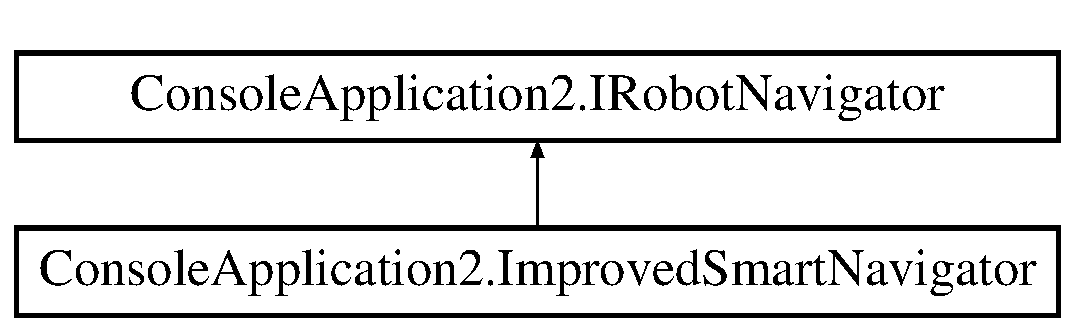
\includegraphics[height=2.000000cm]{class_console_application2_1_1_improved_smart_navigator}
\end{center}
\end{figure}
\subsection*{Public Member Functions}
\begin{DoxyCompactItemize}
\item 
\hypertarget{class_console_application2_1_1_improved_smart_navigator_a66a5460c9224f63e6ad58c92ad114169}{}{\bfseries Improved\+Smart\+Navigator} (\hyperlink{class_console_application2_1_1_vector}{Vector} destination)\label{class_console_application2_1_1_improved_smart_navigator_a66a5460c9224f63e6ad58c92ad114169}

\item 
\hypertarget{class_console_application2_1_1_improved_smart_navigator_aced8a6e0abdc2e8700d6526964f0932e}{}\hyperlink{class_console_application2_1_1_robot_command}{Robot\+Command} {\bfseries Get\+Next\+Command} (\hyperlink{class_console_application2_1_1_robot}{Robot} robot)\label{class_console_application2_1_1_improved_smart_navigator_aced8a6e0abdc2e8700d6526964f0932e}

\end{DoxyCompactItemize}
\subsection*{Static Public Attributes}
\begin{DoxyCompactItemize}
\item 
\hypertarget{class_console_application2_1_1_improved_smart_navigator_a2b7c032e83e36f2fa695f62465fec9f8}{}static double {\bfseries Dt} = 0.\+3\label{class_console_application2_1_1_improved_smart_navigator_a2b7c032e83e36f2fa695f62465fec9f8}

\end{DoxyCompactItemize}


The documentation for this class was generated from the following file\+:\begin{DoxyCompactItemize}
\item 
Improved\+Smart\+Navigator.\+cs\end{DoxyCompactItemize}

\hypertarget{interface_console_application2_1_1_i_noise}{}\section{Console\+Application2.\+I\+Noise Interface Reference}
\label{interface_console_application2_1_1_i_noise}\index{Console\+Application2.\+I\+Noise@{Console\+Application2.\+I\+Noise}}
Inheritance diagram for Console\+Application2.\+I\+Noise\+:\begin{figure}[H]
\begin{center}
\leavevmode
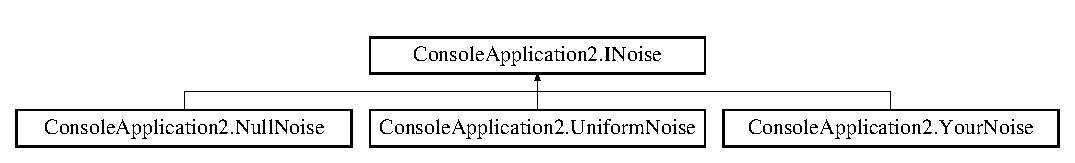
\includegraphics[height=1.736434cm]{interface_console_application2_1_1_i_noise}
\end{center}
\end{figure}
\subsection*{Public Member Functions}
\begin{DoxyCompactItemize}
\item 
\hypertarget{interface_console_application2_1_1_i_noise_a98491fa7488c3c88bd27b1d71c15b014}{}double {\bfseries Noise\+Velocity} (double velocity)\label{interface_console_application2_1_1_i_noise_a98491fa7488c3c88bd27b1d71c15b014}

\end{DoxyCompactItemize}


The documentation for this interface was generated from the following file\+:\begin{DoxyCompactItemize}
\item 
I\+Noise.\+cs\end{DoxyCompactItemize}

\hypertarget{interface_console_application2_1_1_i_robot_navigator}{}\section{Console\+Application2.\+I\+Robot\+Navigator Interface Reference}
\label{interface_console_application2_1_1_i_robot_navigator}\index{Console\+Application2.\+I\+Robot\+Navigator@{Console\+Application2.\+I\+Robot\+Navigator}}
Inheritance diagram for Console\+Application2.\+I\+Robot\+Navigator\+:\begin{figure}[H]
\begin{center}
\leavevmode
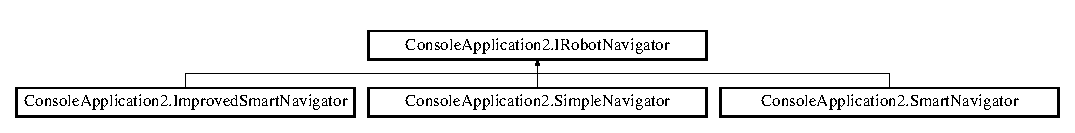
\includegraphics[height=1.338112cm]{interface_console_application2_1_1_i_robot_navigator}
\end{center}
\end{figure}
\subsection*{Public Member Functions}
\begin{DoxyCompactItemize}
\item 
\hypertarget{interface_console_application2_1_1_i_robot_navigator_a7fc80f9689530299e934059713ae2a17}{}\hyperlink{class_console_application2_1_1_robot_command}{Robot\+Command} {\bfseries Get\+Next\+Command} (\hyperlink{class_console_application2_1_1_robot}{Robot} robot)\label{interface_console_application2_1_1_i_robot_navigator_a7fc80f9689530299e934059713ae2a17}

\end{DoxyCompactItemize}


The documentation for this interface was generated from the following file\+:\begin{DoxyCompactItemize}
\item 
I\+Robot\+Navigator.\+cs\end{DoxyCompactItemize}

\hypertarget{class_console_application2_1_1_null_noise}{}\section{Console\+Application2.\+Null\+Noise Class Reference}
\label{class_console_application2_1_1_null_noise}\index{Console\+Application2.\+Null\+Noise@{Console\+Application2.\+Null\+Noise}}
Inheritance diagram for Console\+Application2.\+Null\+Noise\+:\begin{figure}[H]
\begin{center}
\leavevmode
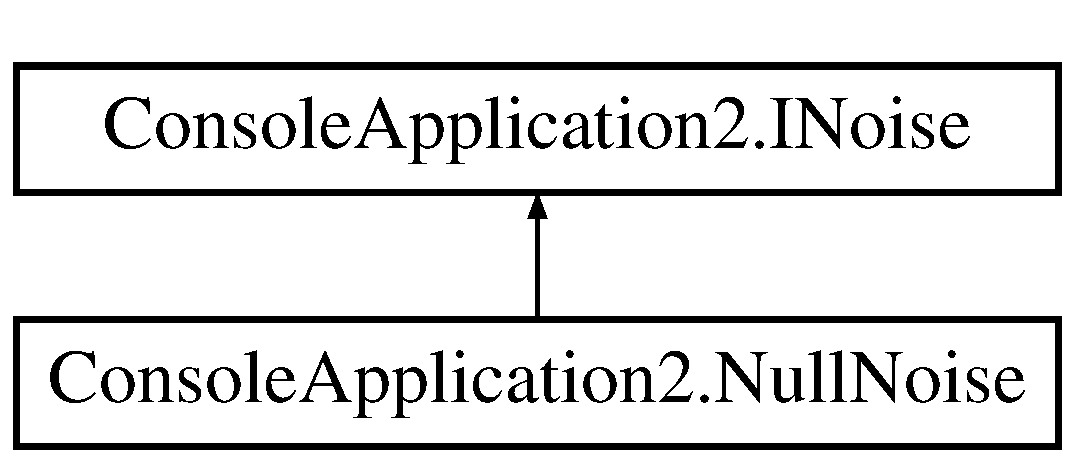
\includegraphics[height=2.000000cm]{class_console_application2_1_1_null_noise}
\end{center}
\end{figure}
\subsection*{Public Member Functions}
\begin{DoxyCompactItemize}
\item 
\hypertarget{class_console_application2_1_1_null_noise_aad85ddd3001ac1aba2953b3e35f14a75}{}double {\bfseries Noise\+Velocity} (double velocity)\label{class_console_application2_1_1_null_noise_aad85ddd3001ac1aba2953b3e35f14a75}

\end{DoxyCompactItemize}


The documentation for this class was generated from the following file\+:\begin{DoxyCompactItemize}
\item 
Null\+Noise.\+cs\end{DoxyCompactItemize}

\hypertarget{class_console_application2_1_1_robot}{}\section{Console\+Application2.\+Robot Class Reference}
\label{class_console_application2_1_1_robot}\index{Console\+Application2.\+Robot@{Console\+Application2.\+Robot}}
\subsection*{Public Member Functions}
\begin{DoxyCompactItemize}
\item 
\hypertarget{class_console_application2_1_1_robot_a7d8dd4df2d0731601425fbd70a33387b}{}{\bfseries Robot} (\hyperlink{class_console_application2_1_1_vector}{Vector} map, \hyperlink{class_console_application2_1_1_angle}{Angle} direction, double max\+Linear\+Velocity, double max\+Angle\+Velocity)\label{class_console_application2_1_1_robot_a7d8dd4df2d0731601425fbd70a33387b}

\item 
\hypertarget{class_console_application2_1_1_robot_a60d751f9edb2e4307bf21066d1ac37d3}{}override string {\bfseries To\+String} ()\label{class_console_application2_1_1_robot_a60d751f9edb2e4307bf21066d1ac37d3}

\item 
\hypertarget{class_console_application2_1_1_robot_a88aaceddaf860b7795cb0c786e591b4c}{}override bool {\bfseries Equals} (object obj)\label{class_console_application2_1_1_robot_a88aaceddaf860b7795cb0c786e591b4c}

\item 
\hypertarget{class_console_application2_1_1_robot_a7dd87bf55a21d40f9672e4f6f8295249}{}\hyperlink{class_console_application2_1_1_robot}{Robot} {\bfseries Move} (\hyperlink{class_console_application2_1_1_robot_command}{Robot\+Command} command, \hyperlink{interface_console_application2_1_1_i_noise}{I\+Noise} noise)\label{class_console_application2_1_1_robot_a7dd87bf55a21d40f9672e4f6f8295249}

\end{DoxyCompactItemize}
\subsection*{Public Attributes}
\begin{DoxyCompactItemize}
\item 
\hypertarget{class_console_application2_1_1_robot_a6277f34887e3e69c1c0d5005d5ac4a77}{}double {\bfseries Max\+Linear\+Velocity}\label{class_console_application2_1_1_robot_a6277f34887e3e69c1c0d5005d5ac4a77}

\item 
\hypertarget{class_console_application2_1_1_robot_a54f03f16f68207310a7fa5802e4e79df}{}double {\bfseries Max\+Angle\+Velocity}\label{class_console_application2_1_1_robot_a54f03f16f68207310a7fa5802e4e79df}

\item 
\hypertarget{class_console_application2_1_1_robot_a53deff1dfc010f58428cf333d157736a}{}double {\bfseries Dt} = 0.\+1\label{class_console_application2_1_1_robot_a53deff1dfc010f58428cf333d157736a}

\end{DoxyCompactItemize}
\subsection*{Properties}
\begin{DoxyCompactItemize}
\item 
\hypertarget{class_console_application2_1_1_robot_a9ddb6c004833053f0dc1d42bc9e026c0}{}\hyperlink{class_console_application2_1_1_vector}{Vector} {\bfseries Map}\hspace{0.3cm}{\ttfamily  \mbox{[}get, set\mbox{]}}\label{class_console_application2_1_1_robot_a9ddb6c004833053f0dc1d42bc9e026c0}

\item 
\hypertarget{class_console_application2_1_1_robot_aa1bb2a94ddd0268ff7138bdcca7eddc8}{}\hyperlink{class_console_application2_1_1_angle}{Angle} {\bfseries Direction}\hspace{0.3cm}{\ttfamily  \mbox{[}get, set\mbox{]}}\label{class_console_application2_1_1_robot_aa1bb2a94ddd0268ff7138bdcca7eddc8}

\end{DoxyCompactItemize}


The documentation for this class was generated from the following file\+:\begin{DoxyCompactItemize}
\item 
Robot.\+cs\end{DoxyCompactItemize}

\hypertarget{class_console_application2_1_1_robot_command}{}\section{Console\+Application2.\+Robot\+Command Class Reference}
\label{class_console_application2_1_1_robot_command}\index{Console\+Application2.\+Robot\+Command@{Console\+Application2.\+Robot\+Command}}
\subsection*{Public Member Functions}
\begin{DoxyCompactItemize}
\item 
\hypertarget{class_console_application2_1_1_robot_command_a45b4b7c8797f4ceda8ce649d252068ec}{}{\bfseries Robot\+Command} (double a, double b, double c)\label{class_console_application2_1_1_robot_command_a45b4b7c8797f4ceda8ce649d252068ec}

\end{DoxyCompactItemize}
\subsection*{Public Attributes}
\begin{DoxyCompactItemize}
\item 
\hypertarget{class_console_application2_1_1_robot_command_a8eb65492e367840067d65708156119cc}{}double {\bfseries Duration}\label{class_console_application2_1_1_robot_command_a8eb65492e367840067d65708156119cc}

\item 
\hypertarget{class_console_application2_1_1_robot_command_a1626bf1f48b38046fb9c3a1294b1730e}{}double {\bfseries Velocity}\label{class_console_application2_1_1_robot_command_a1626bf1f48b38046fb9c3a1294b1730e}

\item 
\hypertarget{class_console_application2_1_1_robot_command_a176b5beecd4a6b844ffcd44e3feee7f9}{}double {\bfseries Angular\+Velocity}\label{class_console_application2_1_1_robot_command_a176b5beecd4a6b844ffcd44e3feee7f9}

\end{DoxyCompactItemize}


The documentation for this class was generated from the following file\+:\begin{DoxyCompactItemize}
\item 
Robot.\+cs\end{DoxyCompactItemize}

\hypertarget{class_console_application2_1_1_scenarios_robot_navigator}{}\section{Console\+Application2.\+Scenarios\+Robot\+Navigator Class Reference}
\label{class_console_application2_1_1_scenarios_robot_navigator}\index{Console\+Application2.\+Scenarios\+Robot\+Navigator@{Console\+Application2.\+Scenarios\+Robot\+Navigator}}
\subsection*{Public Member Functions}
\begin{DoxyCompactItemize}
\item 
\hypertarget{class_console_application2_1_1_scenarios_robot_navigator_acc3d1574d6aa58ef5429be2d6f00b961}{}void {\bfseries scenario} ()\label{class_console_application2_1_1_scenarios_robot_navigator_acc3d1574d6aa58ef5429be2d6f00b961}

\item 
\hypertarget{class_console_application2_1_1_scenarios_robot_navigator_a4d8f87ae455e1aa3f429995cc9d64575}{}void {\bfseries Test} (\hyperlink{class_console_application2_1_1_robot}{Robot} robot, \hyperlink{interface_console_application2_1_1_i_robot_navigator}{I\+Robot\+Navigator} navigator, \hyperlink{class_console_application2_1_1_vector}{Vector} vector, \hyperlink{interface_console_application2_1_1_i_noise}{I\+Noise} noise)\label{class_console_application2_1_1_scenarios_robot_navigator_a4d8f87ae455e1aa3f429995cc9d64575}

\item 
\hypertarget{class_console_application2_1_1_scenarios_robot_navigator_a9853bfbe0703898d4ee8b3121b0926d9}{}void {\bfseries Test\+Smart\+Navigator} (\hyperlink{class_console_application2_1_1_robot}{Robot} robot, \hyperlink{interface_console_application2_1_1_i_robot_navigator}{I\+Robot\+Navigator} navigator, \hyperlink{class_console_application2_1_1_vector}{Vector} vector, \hyperlink{interface_console_application2_1_1_i_noise}{I\+Noise} noise)\label{class_console_application2_1_1_scenarios_robot_navigator_a9853bfbe0703898d4ee8b3121b0926d9}

\end{DoxyCompactItemize}
\subsection*{Static Public Attributes}
\begin{DoxyCompactItemize}
\item 
\hypertarget{class_console_application2_1_1_scenarios_robot_navigator_a488b0381548340360fd8ffeb0e42fee7}{}static double {\bfseries timer} = 0\label{class_console_application2_1_1_scenarios_robot_navigator_a488b0381548340360fd8ffeb0e42fee7}

\end{DoxyCompactItemize}


The documentation for this class was generated from the following file\+:\begin{DoxyCompactItemize}
\item 
Scenarios\+Robot\+Navigator.\+cs\end{DoxyCompactItemize}

\hypertarget{class_console_application2_1_1_simple_navigator}{}\section{Console\+Application2.\+Simple\+Navigator Class Reference}
\label{class_console_application2_1_1_simple_navigator}\index{Console\+Application2.\+Simple\+Navigator@{Console\+Application2.\+Simple\+Navigator}}
Inheritance diagram for Console\+Application2.\+Simple\+Navigator\+:\begin{figure}[H]
\begin{center}
\leavevmode
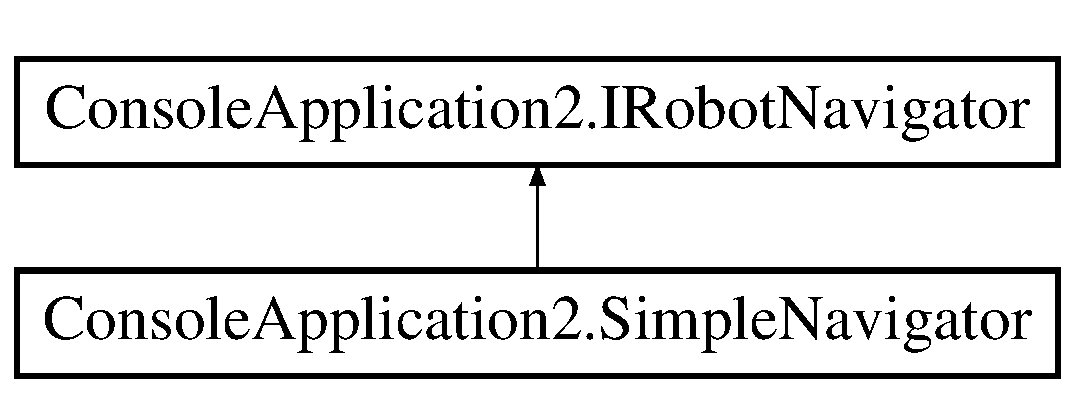
\includegraphics[height=2.000000cm]{class_console_application2_1_1_simple_navigator}
\end{center}
\end{figure}
\subsection*{Public Member Functions}
\begin{DoxyCompactItemize}
\item 
\hypertarget{class_console_application2_1_1_simple_navigator_a362da36b2f55727ed33b2414bb0f5dec}{}{\bfseries Simple\+Navigator} (\hyperlink{class_console_application2_1_1_vector}{Vector} destination)\label{class_console_application2_1_1_simple_navigator_a362da36b2f55727ed33b2414bb0f5dec}

\item 
\hypertarget{class_console_application2_1_1_simple_navigator_a506bed661ee596d9955656dbbee22fce}{}\hyperlink{class_console_application2_1_1_robot_command}{Robot\+Command} {\bfseries Get\+Next\+Command} (\hyperlink{class_console_application2_1_1_robot}{Robot} robot)\label{class_console_application2_1_1_simple_navigator_a506bed661ee596d9955656dbbee22fce}

\end{DoxyCompactItemize}


The documentation for this class was generated from the following file\+:\begin{DoxyCompactItemize}
\item 
Simple\+Navigator.\+cs\end{DoxyCompactItemize}

\hypertarget{class_console_application2_1_1_smart_navigator}{}\section{Console\+Application2.\+Smart\+Navigator Class Reference}
\label{class_console_application2_1_1_smart_navigator}\index{Console\+Application2.\+Smart\+Navigator@{Console\+Application2.\+Smart\+Navigator}}
Inheritance diagram for Console\+Application2.\+Smart\+Navigator\+:\begin{figure}[H]
\begin{center}
\leavevmode
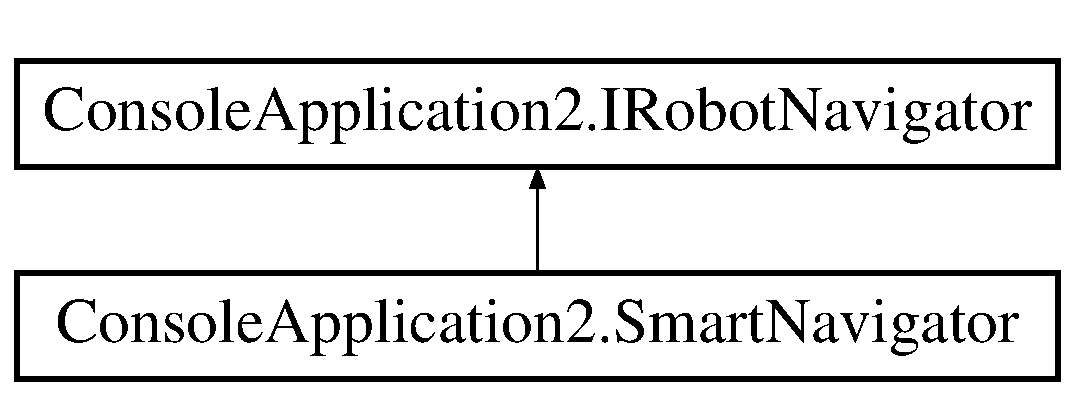
\includegraphics[height=2.000000cm]{class_console_application2_1_1_smart_navigator}
\end{center}
\end{figure}
\subsection*{Public Member Functions}
\begin{DoxyCompactItemize}
\item 
\hypertarget{class_console_application2_1_1_smart_navigator_a9289dd8078b83d28f05de4e942abfae9}{}{\bfseries Smart\+Navigator} (\hyperlink{class_console_application2_1_1_vector}{Vector} destination)\label{class_console_application2_1_1_smart_navigator_a9289dd8078b83d28f05de4e942abfae9}

\item 
\hypertarget{class_console_application2_1_1_smart_navigator_ace757b081a06bdf64cf5ddd7f7e35370}{}\hyperlink{class_console_application2_1_1_robot_command}{Robot\+Command} {\bfseries Get\+Next\+Command} (\hyperlink{class_console_application2_1_1_robot}{Robot} robot)\label{class_console_application2_1_1_smart_navigator_ace757b081a06bdf64cf5ddd7f7e35370}

\end{DoxyCompactItemize}
\subsection*{Static Public Attributes}
\begin{DoxyCompactItemize}
\item 
\hypertarget{class_console_application2_1_1_smart_navigator_af8f0dd2ced3547845bf93c6cb0f44b0c}{}static double {\bfseries Dt} = 0.\+3\label{class_console_application2_1_1_smart_navigator_af8f0dd2ced3547845bf93c6cb0f44b0c}

\end{DoxyCompactItemize}


The documentation for this class was generated from the following file\+:\begin{DoxyCompactItemize}
\item 
Smart\+Navigator.\+cs\end{DoxyCompactItemize}

\hypertarget{class_console_application2_1_1_uniform_noise}{}\section{Console\+Application2.\+Uniform\+Noise Class Reference}
\label{class_console_application2_1_1_uniform_noise}\index{Console\+Application2.\+Uniform\+Noise@{Console\+Application2.\+Uniform\+Noise}}
Inheritance diagram for Console\+Application2.\+Uniform\+Noise\+:\begin{figure}[H]
\begin{center}
\leavevmode
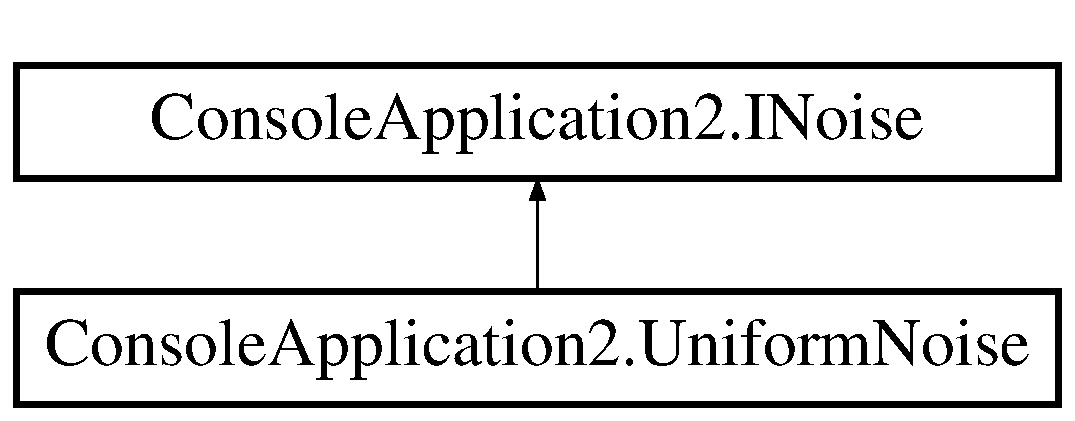
\includegraphics[height=2.000000cm]{class_console_application2_1_1_uniform_noise}
\end{center}
\end{figure}
\subsection*{Public Member Functions}
\begin{DoxyCompactItemize}
\item 
\hypertarget{class_console_application2_1_1_uniform_noise_a53f90382c332a9873325d36076b846d9}{}{\bfseries Uniform\+Noise} (double w)\label{class_console_application2_1_1_uniform_noise_a53f90382c332a9873325d36076b846d9}

\item 
\hypertarget{class_console_application2_1_1_uniform_noise_a0c525817fdc916c31969376abbe3426a}{}double {\bfseries Noise\+Velocity} (double velocity)\label{class_console_application2_1_1_uniform_noise_a0c525817fdc916c31969376abbe3426a}

\end{DoxyCompactItemize}
\subsection*{Properties}
\begin{DoxyCompactItemize}
\item 
\hypertarget{class_console_application2_1_1_uniform_noise_af682171238b2ba6a9ef23f6196b2f10f}{}double {\bfseries W}\hspace{0.3cm}{\ttfamily  \mbox{[}get, set\mbox{]}}\label{class_console_application2_1_1_uniform_noise_af682171238b2ba6a9ef23f6196b2f10f}

\end{DoxyCompactItemize}


The documentation for this class was generated from the following file\+:\begin{DoxyCompactItemize}
\item 
Uniform\+Noise.\+cs\end{DoxyCompactItemize}

\hypertarget{class_console_application2_1_1_vector}{}\section{Console\+Application2.\+Vector Class Reference}
\label{class_console_application2_1_1_vector}\index{Console\+Application2.\+Vector@{Console\+Application2.\+Vector}}
\subsection*{Public Member Functions}
\begin{DoxyCompactItemize}
\item 
\hypertarget{class_console_application2_1_1_vector_a2c3bbdbecc7fbd0b1e12e842850cb41a}{}{\bfseries Vector} (double x, double y)\label{class_console_application2_1_1_vector_a2c3bbdbecc7fbd0b1e12e842850cb41a}

\item 
\hypertarget{class_console_application2_1_1_vector_a39cd2e4386c7600534f07e90f40da297}{}\hyperlink{class_console_application2_1_1_vector}{Vector} {\bfseries Subtract} (\hyperlink{class_console_application2_1_1_vector}{Vector} v)\label{class_console_application2_1_1_vector_a39cd2e4386c7600534f07e90f40da297}

\item 
\hypertarget{class_console_application2_1_1_vector_a92fe1c9da508aeb518f5da33d5429eae}{}\hyperlink{class_console_application2_1_1_vector}{Vector} {\bfseries Add} (\hyperlink{class_console_application2_1_1_vector}{Vector} v)\label{class_console_application2_1_1_vector_a92fe1c9da508aeb518f5da33d5429eae}

\item 
\hypertarget{class_console_application2_1_1_vector_a90aee8f0883398df708c1025443b6b60}{}\hyperlink{class_console_application2_1_1_vector}{Vector} {\bfseries Multiply} (double a)\label{class_console_application2_1_1_vector_a90aee8f0883398df708c1025443b6b60}

\item 
\hypertarget{class_console_application2_1_1_vector_abde9e17b0195853e84b9f7515558f533}{}double {\bfseries Len} ()\label{class_console_application2_1_1_vector_abde9e17b0195853e84b9f7515558f533}

\item 
\hypertarget{class_console_application2_1_1_vector_afccb46386f90449c592beb995fa0309c}{}double {\bfseries Len\+Two\+Vectors} (\hyperlink{class_console_application2_1_1_vector}{Vector} vector)\label{class_console_application2_1_1_vector_afccb46386f90449c592beb995fa0309c}

\item 
\hypertarget{class_console_application2_1_1_vector_a83828a23f1a3938f05c0d2afb5d0c8bb}{}override bool {\bfseries Equals} (object obj)\label{class_console_application2_1_1_vector_a83828a23f1a3938f05c0d2afb5d0c8bb}

\item 
\hypertarget{class_console_application2_1_1_vector_a652f7596db2c6fe1c6bb28a399d6ffc1}{}override string {\bfseries To\+String} ()\label{class_console_application2_1_1_vector_a652f7596db2c6fe1c6bb28a399d6ffc1}

\item 
\hypertarget{class_console_application2_1_1_vector_aa6ffae8d1611d9fdf8805f945889df86}{}override int {\bfseries Get\+Hash\+Code} ()\label{class_console_application2_1_1_vector_aa6ffae8d1611d9fdf8805f945889df86}

\end{DoxyCompactItemize}
\subsection*{Properties}
\begin{DoxyCompactItemize}
\item 
\hypertarget{class_console_application2_1_1_vector_a80fde222448cb457c273e5c58448b974}{}double {\bfseries X}\hspace{0.3cm}{\ttfamily  \mbox{[}get\mbox{]}}\label{class_console_application2_1_1_vector_a80fde222448cb457c273e5c58448b974}

\item 
\hypertarget{class_console_application2_1_1_vector_ae9522fa1917a1201a2ce3e450ad304d3}{}double {\bfseries Y}\hspace{0.3cm}{\ttfamily  \mbox{[}get\mbox{]}}\label{class_console_application2_1_1_vector_ae9522fa1917a1201a2ce3e450ad304d3}

\end{DoxyCompactItemize}


The documentation for this class was generated from the following file\+:\begin{DoxyCompactItemize}
\item 
Program.\+cs\end{DoxyCompactItemize}

\hypertarget{class_console_application2_1_1_your_noise}{}\section{Console\+Application2.\+Your\+Noise Class Reference}
\label{class_console_application2_1_1_your_noise}\index{Console\+Application2.\+Your\+Noise@{Console\+Application2.\+Your\+Noise}}
Inheritance diagram for Console\+Application2.\+Your\+Noise\+:\begin{figure}[H]
\begin{center}
\leavevmode
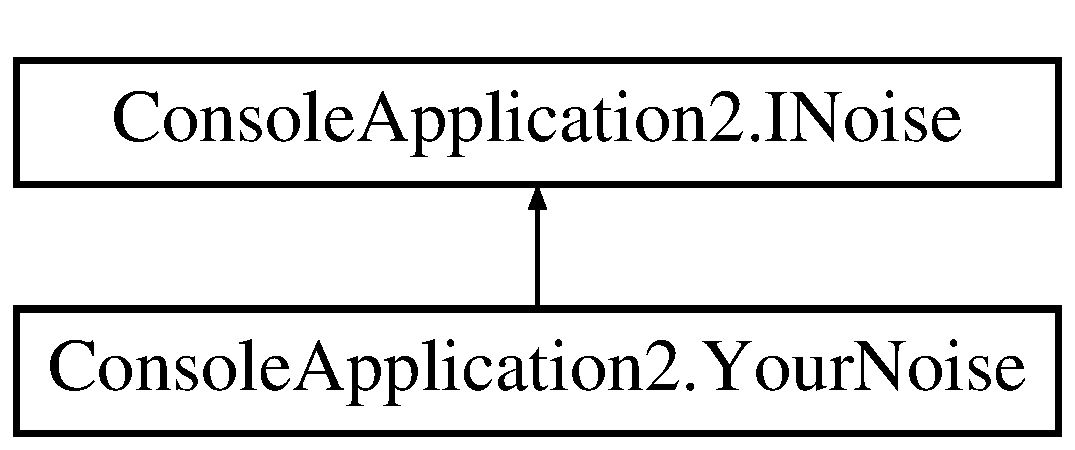
\includegraphics[height=2.000000cm]{class_console_application2_1_1_your_noise}
\end{center}
\end{figure}
\subsection*{Public Member Functions}
\begin{DoxyCompactItemize}
\item 
\hypertarget{class_console_application2_1_1_your_noise_ab1e4461e963ea2eec83176533285d6bf}{}{\bfseries Your\+Noise} (double w)\label{class_console_application2_1_1_your_noise_ab1e4461e963ea2eec83176533285d6bf}

\item 
\hypertarget{class_console_application2_1_1_your_noise_a64822728bc3ba430397487dfeca189c7}{}double {\bfseries Noise\+Velocity} (double velocity)\label{class_console_application2_1_1_your_noise_a64822728bc3ba430397487dfeca189c7}

\end{DoxyCompactItemize}
\subsection*{Properties}
\begin{DoxyCompactItemize}
\item 
\hypertarget{class_console_application2_1_1_your_noise_a8f65e201a9ed900a30c3bdafbc6e9eb9}{}double {\bfseries W}\hspace{0.3cm}{\ttfamily  \mbox{[}get, set\mbox{]}}\label{class_console_application2_1_1_your_noise_a8f65e201a9ed900a30c3bdafbc6e9eb9}

\end{DoxyCompactItemize}


The documentation for this class was generated from the following file\+:\begin{DoxyCompactItemize}
\item 
Your\+Noise.\+cs\end{DoxyCompactItemize}

%--- End generated contents ---

% Index
\backmatter
\newpage
\phantomsection
\clearemptydoublepage
\addcontentsline{toc}{chapter}{Index}
\printindex

\end{document}
